%
%===============>>  ГРУППА 11-6 МОДУЛЬ 4  <<=============
%
\setmodule{4}
%
%===============>>  Занятие 1  <<===============
%
\begin{class}[number=1]
	\begin{listofex}
		\item Упростить:
		\begin{enumcols}[itemcolumns=4]
			\item \( \sin(90\degree-x) \)
			\item \( \cos(360\degree + x) \)
			\item \( \tg(180\degree+x) \)
			\item \( \cos(810\degree-x) \)
		\end{enumcols}
		\item Вычислить:
		\begin{enumcols}[itemcolumns=2]
			\item \( \dfrac{\sqrt{3}}{\sin60\degree}+\dfrac{3}{\sin30\degree} \)
			\item \( \dfrac{17\sin155\degree}{\sin25\degree} \)
			\item \( \dfrac{-2\sin105\degree}{\cos15\degree} \)
			\item \( \sin^215\degree-1+\cos^215 \)
			\item \( -\sqrt{27}\cos30\degree-\sqrt{2}\sin45\degree\ctg60\degree\tg60\degree\)
			\item \( \dfrac{9\sin45\degree\cos45\degree}{\cos^245\degree-\sin^245\degree} \)
		\end{enumcols}
		\item Вычислить:
		\begin{enumcols}[itemcolumns=2]
			\item \( \sin240\degree\sin150\degree\sin(-90)\degree\tg30\degree \)
			\item \( \cos(-300\degree)\sin(-120\degree)\tg(-150\degree) \)
		\end{enumcols}
		\item Упростить:
		\begin{enumcols}[itemcolumns=4]
			\item \( \sin\left( \dfrac{\pi}{2}+x \right) \)
			\item \( \cos(\pi+x) \)
			\item \( \tg\left( \dfrac{3\pi}{2}-x \right) \)
			\item \( \sin(-3,5\pi-x) \)
		\end{enumcols}
		\item Вычислить:
		\begin{enumcols}[itemcolumns=2]
			\item \( \sin\dfrac{5\pi}{4}\cos\dfrac{4\pi}{3}\tg\dfrac{2\pi}{3}\ctg\dfrac{3\pi}{4} \)
			\item \( \cos\left( -\dfrac{5\pi}{3} \right)\sin\left( -\dfrac{5\pi}{2} \right)\sin\dfrac{3\pi}{2} \)
		\end{enumcols}
		\item Площадь треугольника можно вычислить по формуле \( S=\dfrac{bc\sin \alpha}{2} \),  где \( b \)  и \( c \)  --- стороны треугольника, а  \( \alpha \) --- угол между этими сторонами. Пользуясь этой формулой, найдите площадь треугольника, если  \( \alpha = 30\degree \), \( c = 5 \), \( b = 6 \).
		\item Длина биссектрисы \( l_c \), проведенной к стороне c треугольника со сторонами \( a \), \( b \) и \( c \), вычисляется по формуле \( l_c=\sqrt{ab\left( 1-\dfrac{c^2}{(a+b)^2} \right)} \). Треугольник имеет стороны \( 9 \), \( 18 \) и \( 21 \). Найдите длину биссектрисы, проведённой к стороне длины \( 21 \).
		\item Одного рулона обоев хватает для оклейки полосы от пола до потолка шириной \( 2 \) м. Сколько рулонов обоев нужно купить для оклейки прямоугольной комнаты размерами \( 2,1 \) м на \( 3,2 \) м?
		\item Расписание поездов Москва–Минск и стоимость билетов представлены в таблице.
		\begin{center}
			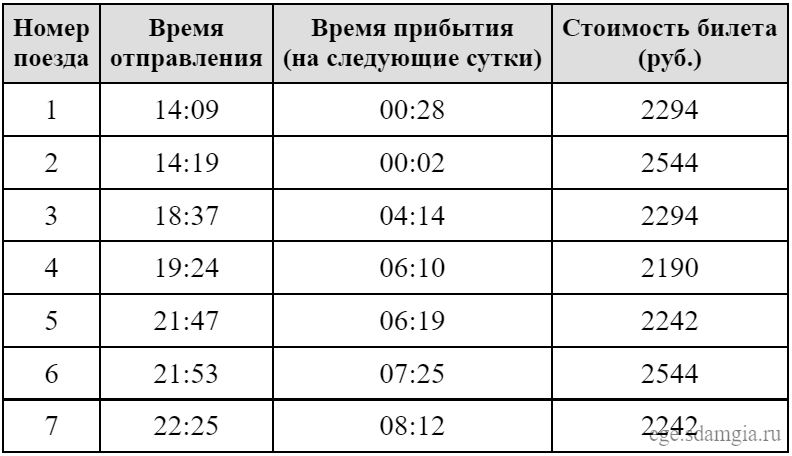
\includegraphics[align=t, width=0.3\textwidth]{pics/G116M4L1-1}
		\end{center}
		Алексей хочет купить пылесос в магазине, который находится не дальше \( 1,4 \) км от его дома. Найдите наименьшую стоимость пылесоса в магазинах (из представленных), удовлетворяющих данному условию. Ответ дайте в рублях.
	\end{listofex}
\end{class}
%
%===============>>  Занятие 2  <<===============
%
%\begin{class}[number=2]
%	\begin{listofex}
%		\item Пусто
%	\end{listofex}
%\end{class}
%
%===============>>  Домашняя работа 1  <<===============
%
%\begin{homework}[number=1]
%	\begin{listofex}
%		\item Пусто
%	\end{listofex}
%\end{homework}
%
%===============>>  Занятие 3  <<===============
%
%\begin{class}[number=3]
%	\begin{listofex}
%		\item Пусто
%	\end{listofex}
%\end{class}
%
%===============>>  Занятие 4  <<===============
% смещение на одно занятие с прошлого месяца
%\begin{class}[number=4]
%	\begin{listofex}
%		\item Пусто
%	\end{listofex}
%\end{class}
%
%===============>>  Домашняя работа 2  <<===============
%
%\begin{homework}[number=2]
%	\begin{listofex}
%
%	\end{listofex}
%\end{homework}
%
%===============>>  Занятие 5  <<===============
% смещение на одно занятие с прошлого месяца
%\begin{class}[number=5]
%	\begin{listofex}
%		\item Пусто
%	\end{listofex}
%\end{class}
%
%===============>>  Домашняя работа 3  <<===============
%
%\begin{homework}[number=2]
%	\begin{listofex}
%
%	\end{listofex}
%\end{homework}
%\newpage
%\title{Подготовка к проверочной работе}
%\begin{listofex}
%	
%\end{listofex}
%
%===============>>  Занятие 7  <<===============
%
%\begin{class}[number=7]
%	\begin{listofex}
%	
%	\end{listofex}
%\end{class}
%
%===============>>  Провечная работа  <<===============
%
%\begin{exam}
%	\begin{listofex}
%	
%	\end{listofex}
%\end{exam}